\begin{figure}[ht!]
  \begin{subfigure}[c]{\textwidth}
    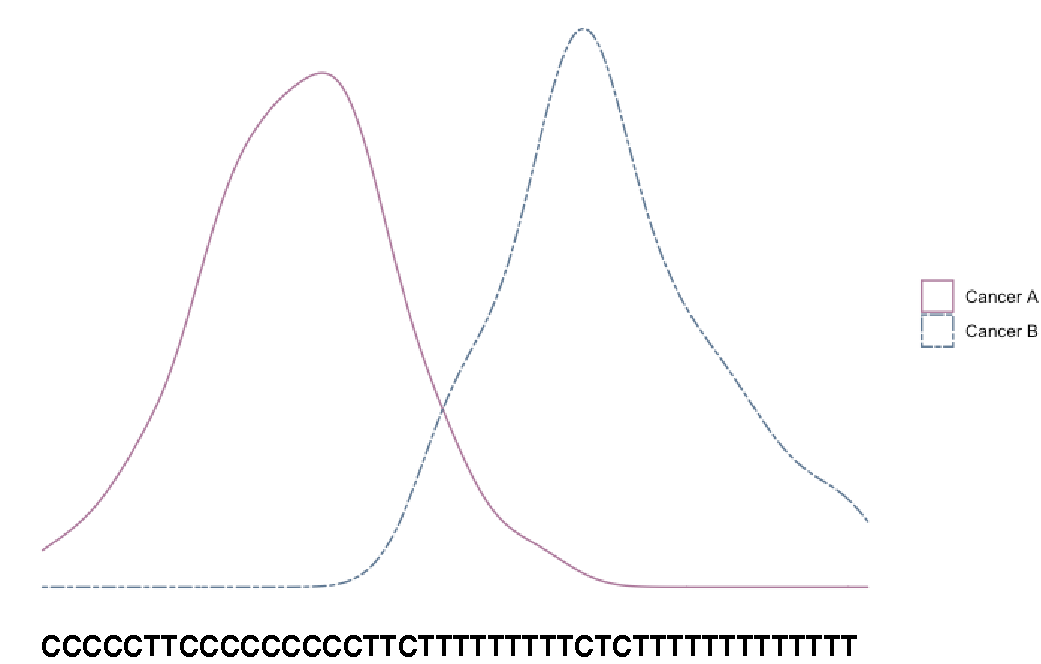
\includegraphics[scale=0.9]{graphics/discussion_gle.pdf}
    \caption{Mutation density of a hypothetical genomic region}
  \end{subfigure}\hfill
  \vspace{1cm}
  
  \begin{subfigure}[c]{0.48\textwidth}
  \centering
    \begin{tabulary}{\columnwidth}{rRR}
    \toprule
        & \textbf{A/T mutated (Cancer A)} &  \textbf{C/G mutated (Cancer A)} \\
    \hline
        \textbf{closed} & $c_{AT}$ &  $c_{CG}$ \\
        \textbf{open} & $o_{AT}$ & $o_{CG}$  \\
    \bottomrule
    \end{tabulary}
    \caption{AT/CG mutation distribution in 1 cancer}
  \end{subfigure}\hfill
  \begin{subfigure}[c]{0.48\textwidth}
    \begin{tabulary}{\columnwidth}{rRR}
    \toprule
        & \textbf{A/T mutated (Cancer A)} &  \textbf{A/T mutated (Cancer B)} \\
    \hline
        \textbf{closed} & $c_{A}$ &  $c_{B}$ \\
        \textbf{open} & $o_{A}$ & $o_{B}$  \\
    \bottomrule
    \end{tabulary}
    \caption{AT mutation distribution across 2 cancers}
  \end{subfigure}
  \vspace{0.8cm}
  
  \begin{minipage}[c]{\textwidth}
    \caption{
      \textbf{Proposed explanation for why GLE differ between Cancer A and Cancer B.} Cancer A is under the influence of a mutagen that targets the base C; Cancer B is under the influence of a mutagen that targets the base T. Panel (a) Some regions of the genome are more enriched in C, others are enriched in T. The distribution of bases combines with chromatin structure to influence GLE. This could be evaluated by assessing (b) whether certain substitutions are enriched in closed/open chromatin regions, or whether (c) two cancers differ in how mutations with wildtype A/T are distributed between closed/open chromatin regions, as per the tables underneath the figure - the techniques are similar to those described in Methods \ref{methods:chromatin}.
    } \label{fig:discussion_gle}
  \end{minipage}
\end{figure}
